\section{
    Формулировка теоремы про ЖНФ. Алгоритм построения ЖНФ. Определение количества клеток. Нахождение базиса. 
}

\begin{theorem}
    Пусть $\lambda_1, \lambda_2, \ldots$ – все собственные числа (корни характеристического уравнения) оператора $\mathscr{A}$, действующего в $n$-мерном пространстве $\mathcal{L}$. Тогда в $\mathcal{L}$ существует базис, в котором матрица оператора имеет блочно-диагональный вид $A_J = J_1 \oplus J_2 \oplus \ldots \oplus J_s$, т.е. является прямой суммой жордановых клеток (блоков), каждая из которых является квадратной матрицей, на главной диагонали которой стоят одинаковые числа $\lambda_i$, над диагональю стоят единицы, а все остальные элементы равны нулю:

    \begin{figure}[H]
        \centering
        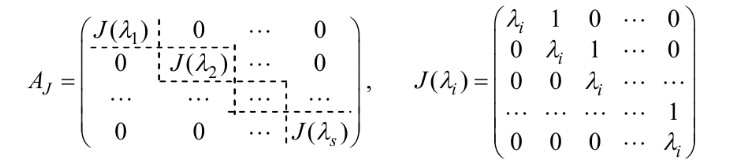
\includegraphics[scale=0.7]{images/27_1.jpg}
        \label{fig:picture_27_1}
    \end{figure} 
\end{theorem}

